\documentclass[conference]{IEEEtran}
\usepackage[T1]{fontenc}
\usepackage{graphicx}
\usepackage{booktabs}
\usepackage{amsmath,amssymb}
\usepackage{url}
\usepackage[hidelinks]{hyperref}
\usepackage{xcolor}

\graphicspath{{figures/}}

\begin{document}

\title{Can a Model Tell Cause from Correlation?\\
Phase 2: Reading Reworded Text with a Transformer}

\author{
\IEEEauthorblockN{Chaitanya Sai Meka, Rakshita, Dhanvin Vadlamudi, Kasula Lalithendra, Jagruthi Pulumati}
\IEEEauthorblockA{CSAI Project, Phase 2 (Deep Learning)\\
Code: \url{https://github.com/Jag2007/AI_ML_Project}}
}

\maketitle

\begin{abstract}
In Phase 1 we built a pipeline that reads Corr2Cause text with regex, turns it into a causal graph with the PC
algorithm, and decides if a causal claim is valid (test F1 0.957). Regex only works because the dataset uses a few
fixed sentences. In Phase 2 we test the pipeline on the dataset authors' two harder test sets, where the claims are
reworded or the variables renamed. The Phase 1 regex reads none of the reworded claims (F1 0.00). We fine-tune a
DistilBERT transformer to read the claim and keep the PC graph for the reasoning. This pipeline keeps an F1 of 0.95
on all three test sets, and the graphs it builds from reworded text still answer 28 of 32 ``what if'' questions
correctly. A DistilBERT that reads the whole text and uses no graph reaches only 0.53, and falls to 0.39 and 0.29 on
the harder sets. So fluent language alone is not causal reasoning.
\end{abstract}

\section{Introduction}
\textbf{The task.} Corr2Cause~\cite{jin2024} gives a short text (the premise) that says which variables are
correlated or independent, and a cause-and-effect claim (the hypothesis), such as ``A directly causes B''. The label
is 1 only if the claim is true in \emph{every} causal graph that fits the premise.

\textbf{What Phase 1 did.} Five notebooks, one per team member: (01) clean the data and remove leakage, (02) read
the text with regex and build the causal graph with the PC algorithm, (03) build TF-IDF and graph features, (04)
train and pick a classifier, and (05) build a DAG and ask a Bayesian network ``what if'' questions.
Table~\ref{tab:phase1} lists the main results.

\begin{table}[t]
\centering
\caption{Phase 1 results on the original test set}
\label{tab:phase1}
\begin{tabular}{lc}
\toprule
What we measured & Result \\
\midrule
Symbolic rule (graph only, no learning): F1 & 0.952 \\
Random Forest (chosen on validation): F1 & 0.957 \\
TF-IDF features only (validation): F1 & 0.47 \\
Edge precision of the predicted DAGs & 0.89 \\
Real ``what if'' effects answered correctly & 28 / 32 \\
\bottomrule
\end{tabular}
\end{table}

\textbf{The gap.} Phase 1 reads the text with regex, which only works because Corr2Cause uses a few fixed sentence
templates. The Corr2Cause authors also made two harder copies of the test set to check if a model really reasons:
\begin{itemize}
\item \textbf{Paraphrasing:} every claim is reworded, for example ``A directly causes B'' becomes ``A directly
affects B''.
\item \textbf{Refactorization:} the variables are renamed, for example A, B, C become Z, Y, X.
\end{itemize}
They found that fine-tuned language models break down on both. Phase 2 asks: can a transformer read the claims
while the PC graph still does the reasoning? We compare four methods on all three test sets
(Table~\ref{tab:methods}).

\begin{table}[t]
\centering
\caption{The four methods compared in Phase 2}
\label{tab:methods}
\footnotesize
\setlength{\tabcolsep}{3pt}
\begin{tabular}{p{0.36\linewidth}p{0.30\linewidth}p{0.24\linewidth}}
\toprule
Method & Reads the claim with & Reasoning \\
\midrule
Phase 1 pipeline & Regex & PC graph \\
Classical ML reader & TF-IDF + logistic regression & PC graph \\
Transformer reader & Fine-tuned DistilBERT & PC graph \\
End-to-end transformer & DistilBERT reads everything & None \\
\bottomrule
\end{tabular}
\end{table}

All graph methods decide with the Phase 1 \emph{symbolic rule}: a claim is valid if it holds in every fitting DAG
(mec\_support $=1$, Section~\ref{sec:ideas}). In Phase 1 the Random Forest beat this rule by only 0.005 F1, inside
the confidence interval, so in Phase 2 the comparison is only about \emph{reading}.

\section{Related Work}
\textbf{Bayesian networks.} Pearl~\cite{pearl1988} introduced Bayesian networks: a DAG with a probability table at
each node. We use them to answer ``what if'' (intervention) questions.

\textbf{Transformers.} BERT~\cite{devlin2019} is a transformer language model that is first trained on a lot of
plain text and then \emph{fine-tuned} on a small labelled task. DistilBERT~\cite{sanh2019} is a smaller copy of
BERT (6 layers instead of 12) that keeps about 97\% of its language understanding and runs about 60\% faster, so it
can be fine-tuned on a free GPU.

\textbf{Language models on Corr2Cause.} The Corr2Cause authors~\cite{jin2024} found that fine-tuned models score
well on the original test but fail on the reworded and renamed versions, so they learn surface patterns, not
reasoning.

\textbf{Neuro-symbolic AI.} A learned part reads the input and a rule-based part does exact
reasoning~\cite{garcez2023}. Phase 2 makes the learned part a transformer and keeps the graph.

\section{Key Ideas}
\label{sec:ideas}
\textbf{mec\_support.} Many DAGs can fit one premise. For each claim we count in how many of them it is true:
\begin{equation}
\text{mec\_support} = \frac{\text{fitting DAGs where the claim is true}}{\text{all fitting DAGs}}.
\end{equation}
If mec\_support $=1$, the claim holds in every fitting DAG, so we call it valid.

\textbf{Transformer, token and fine-tuning.} A transformer reads a sentence as a list of \emph{tokens} (words or
pieces of words) and looks at all of them together, including their order. DistilBERT reads at most 512 tokens at
once. \emph{Fine-tuning} means we start from the pretrained model, add a small new output layer, and train the whole
model for a short time on our own examples.

\textbf{Intervention.} Forcing a variable to a value is written $do(X)$. The effect of X on Y is
\begin{equation}
\text{effect} = P(Y{=}1 \mid do(X{=}1)) - P(Y{=}1 \mid do(X{=}0)).
\end{equation}

\textbf{Evaluation.} From the confusion matrix (TP, FP, FN, TN):
\begin{equation}
P = \frac{TP}{TP+FP},\quad R = \frac{TP}{TP+FN},\quad F_1 = \frac{2PR}{P+R}.
\end{equation}
Precision: of the claims we called valid, how many really were. Recall: of the truly valid claims, how many we found.

\section{Step 6: The Harder Test Sets (Notebook 06)}
We loaded both sets (2{,}246 rows each) and cleaned them like the original data in Phase 1. There were no missing values. The paraphrasing
set uses three labels (entailment, neutral, contradiction); only entailment means ``valid'', so we turned it into
1/0. About 15\% of the claims are valid in all three test sets.

\textbf{Entity schema.} We rename the variables by the order the premise lists them: the first variable becomes A,
the second B, and so on. So ``Z, Y and X'' becomes ``A, B and C'' in both the premise and the claim. This is one
fixed rule that keeps our variable names to A--F. After renaming, both sets use exactly the same 21 premises as our
original test set and none of the train or validation premises, so there is no leakage.

\textbf{New wordings.} Each claim type gets one new wording in the paraphrasing set (Table~\ref{tab:wordings}).
The regex parser knows none of them.

\begin{table}[t]
\centering
\caption{The same claims in the original and the paraphrasing test sets}
\label{tab:wordings}
\footnotesize
\setlength{\tabcolsep}{3pt}
\begin{tabular}{p{0.44\linewidth}p{0.48\linewidth}}
\toprule
Original & Paraphrasing \\
\midrule
A directly causes B. & A directly affects B. \\
A causes something else which causes B. & A influences B through some mediator(s). \\
There exists at least one collider (i.e., common effect) of A and B. & A and B together cause some other
variable(s). \\
There exists at least one confounder (i.e., common cause) of A and B. & Some variable(s) cause(s) both A and B. \\
\bottomrule
\end{tabular}
\end{table}

\section{Step 7: Reading the Claim (Notebook 07)}
A \emph{reader} takes the claim sentence and predicts its type: direct cause, indirect cause, collider or
confounder. The two variables are still the single capital letters. We compare three readers.

\textbf{Training sentences.} The readers learn from sentences only, never from labels. Trained on the five
original templates alone, TF-IDF read only 75\% and DistilBERT only 50\% of new wordings we held out, so five
wordings are not enough. We therefore wrote four extra wordings for each claim type, such as ``A and B share a
common effect''. None of them uses the words of the authors' test (``affects'', ``influences'', ``mediator'',
``together''). Filled in with every pair of A--F this gives 600 training sentences, plus 120 validation
sentences from one more held-out wording per type.

\textbf{The readers.} The \emph{classical ML reader} is TF-IDF with logistic regression. The \emph{transformer
reader} is DistilBERT fine-tuned for 3 epochs (learning rate $3\times10^{-5}$, batch size 16, seed 42).

\begin{table}[t]
\centering
\caption{Share of test claims each reader reads correctly}
\label{tab:readers}
\begin{tabular}{lccc}
\toprule
Reader & Original & Paraphrasing & Refactorization \\
\midrule
Regex (Phase 1) & 100\% & 0\% & 100\% \\
TF-IDF + LR & 100\% & 66.8\% & 100\% \\
\textbf{DistilBERT} & \textbf{100\%} & \textbf{100\%} & \textbf{100\%} \\
\bottomrule
\end{tabular}
\end{table}

\begin{figure}[t]
\centering
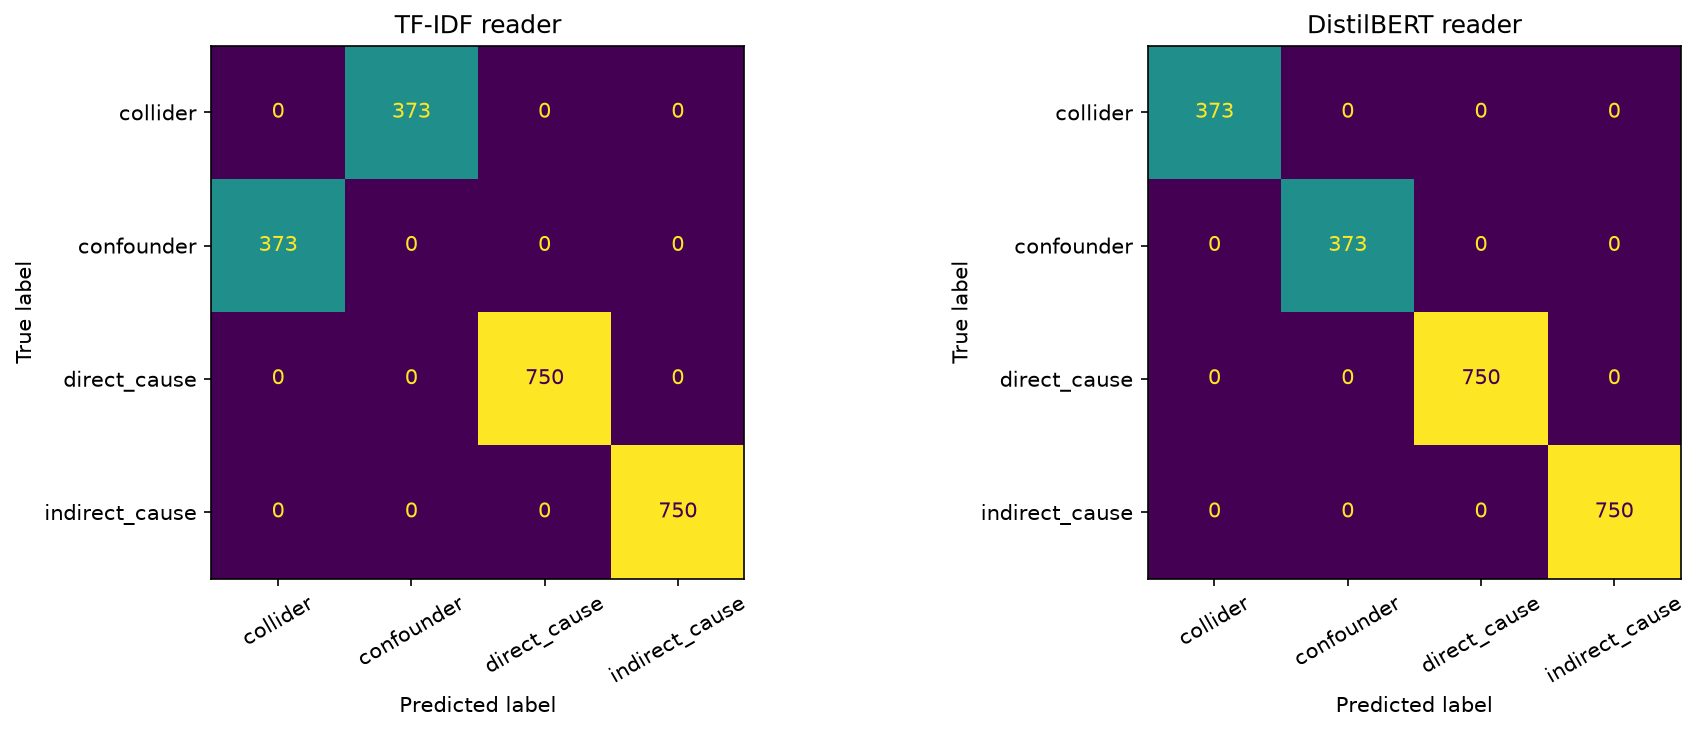
\includegraphics[width=\linewidth]{reader_confusion}
\caption{Claim types read on the paraphrasing set. TF-IDF swaps every collider and confounder; DistilBERT reads
all of them correctly.}
\label{fig:readers}
\end{figure}

\textbf{Results.} Table~\ref{tab:readers} and Fig.~\ref{fig:readers} show the results. On the reworded claims the
regex reads nothing. TF-IDF gets direct and indirect causes right but scores precision, recall and F1 of 0 on
colliders and confounders (macro F1 0.50): ``A and B together cause some other variable'' (collider) and ``Some
variable causes both A and B'' (confounder) use almost the same words in a different order, and TF-IDF only counts
words. DistilBERT reads words in order, so it gets precision, recall and F1 of 1.00 for every type.

\textbf{Review of unsure reads.} We only pass a read straight to the graph step when DistilBERT is at least 90\%
sure. This covers 90\% of the reworded claims, and every one of them is right; the rest would go to a person.

\textbf{Seed check.} Fine-tuning on 600 short sentences depends on the random start. With three other seeds
DistilBERT read 83--91\% of the reworded claims (100\% with seed 42), always above TF-IDF (67\%). We report this
range, not just the best run, and keep seed 42 as in Phase 1.

\section{Step 8: End-to-End DistilBERT (Notebook 08)}
This is the ``language only'' model: DistilBERT reads the premise and the claim together and says valid or not,
with no parser and no graph. We fine-tuned it on the same 35{,}340 train rows as Phase 1 for one epoch (batch size
8, learning rate $3\times10^{-5}$, balanced class weights), which took 31 minutes on a free Google Colab T4 GPU.

\textbf{The 512-token limit.} 160 of the 400 train premises are longer than 512 tokens, so DistilBERT only sees
their first part. We cut the premise and always keep the claim. The test premises are shorter and fit. Our graph
pipeline has no such limit.

\begin{table}[t]
\centering
\caption{End-to-end DistilBERT on the three test sets}
\label{tab:e2e}
\begin{tabular}{lccc}
\toprule
Test set & Precision & Recall & F1 \\
\midrule
Original & 0.367 & 0.939 & 0.528 \\
Paraphrasing & 0.301 & 0.547 & 0.388 \\
Refactorization & 0.204 & 0.529 & 0.294 \\
\bottomrule
\end{tabular}
\end{table}

\textbf{Results.} Validation F1 is only 0.49, and test F1 is 0.53 on the original wording, falling to 0.39 and
0.29 on the harder sets (Table~\ref{tab:e2e}). The model calls about 40\% of claims valid when only 15\% are: on the
original test it makes 291 false alarms but misses only 11 valid claims. Renaming the variables back to A--F lifts
its refactorization F1 from 0.29 to 0.51, so it partly relies on the letter names it saw in training. It has
learned word patterns, not the rule ``true in every fitting DAG''. This matches what the Corr2Cause authors found.

\section{Step 9: Comparison (Notebook 09)}
Table~\ref{tab:compare} and Fig.~\ref{fig:compare} put all four methods side by side.

\begin{table}[t]
\centering
\caption{Test F1 of every method on the three test sets}
\label{tab:compare}
\setlength{\tabcolsep}{4pt}
\begin{tabular}{lccc}
\toprule
Method & Original & Paraphr. & Refactor. \\
\midrule
Regex + PC (Phase 1) & 0.952 & 0.000 & 0.948 \\
TF-IDF reader + PC & 0.952 & 0.536 & 0.948 \\
\textbf{DistilBERT reader + PC} & \textbf{0.952} & \textbf{0.948} & \textbf{0.948} \\
End-to-end DistilBERT & 0.528 & 0.388 & 0.294 \\
\bottomrule
\end{tabular}
\end{table}

\begin{figure}[t]
\centering
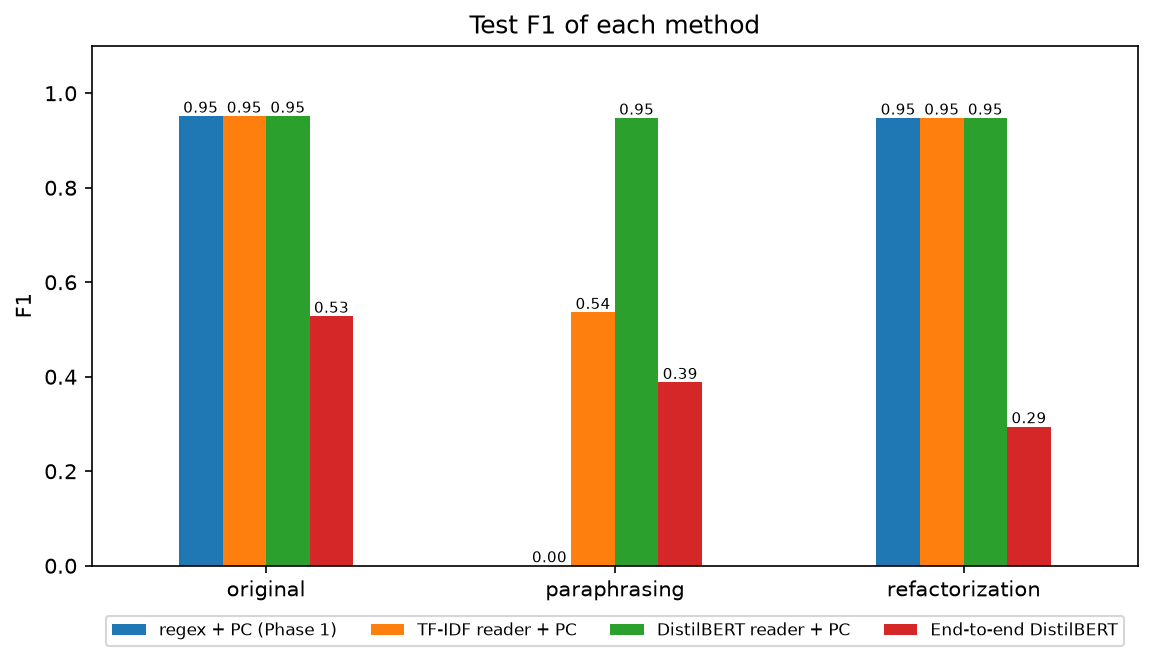
\includegraphics[width=\linewidth]{comparison_f1}
\caption{Test F1 of each method. Only the DistilBERT reader with the PC graph stays high on all three test sets.}
\label{fig:compare}
\end{figure}

\textbf{Renaming.} Without our renaming rule, the Phase 1 regex (which only allows A--F) misses every independence
in the renamed premises and scores F1 0.00 on refactorization. With it, the regex pipeline scores 0.948.

\textbf{Confidence intervals.} With a bootstrap over premises, as in Phase 1, the DistilBERT pipeline's 95\% interval is
0.91--0.98 on the original test and 0.91--0.98 on both harder sets. The end-to-end model's is 0.38--0.62,
0.27--0.47 and 0.20--0.36. The intervals never overlap.

\textbf{Error analysis.} Every mistake of the DistilBERT pipeline (18 on the original test, 37 on each harder set)
is a claim it \emph{read correctly}. So reading is no longer the problem: the remaining mistakes are the label
disagreements found in Phase 1.

\section{Step 10: Graphs from Reworded Text (Notebook 10)}
We repeated the Phase 1 DAG step (notebook 05) on the paraphrasing set. Every ``X directly affects Y'' claim that the DistilBERT pipeline calls
valid, and that DistilBERT read with at least 90\% confidence, becomes an arrow (all 138 were confident, so none
had to wait for review). The same rules skip self-loops, unknown variables and cycles, so all 21 graphs are DAGs.

\textbf{Results.} We drew 73 arrows and 65 are correct: \textbf{edge precision 0.89 and recall 1.00}, exactly the
Phase 1 graphs. On the five fully known premises the graphs answer \textbf{28 of the 32} real intervention effects
correctly (92 of 96 queries). The regex reader finds no arrows in the reworded text, so its graphs are empty and
it gets 0 of the 32 real effects.


\section{What Improved from Phase 1}
Table~\ref{tab:improved} puts the two phases side by side.

\begin{table}[t]
\centering
\caption{Phase 1 vs Phase 2}
\label{tab:improved}
\footnotesize
\setlength{\tabcolsep}{3pt}
\begin{tabular}{p{0.30\linewidth}p{0.28\linewidth}p{0.32\linewidth}}
\toprule
 & Phase 1 & Phase 2 \\
\midrule
Reads the claim with & Regex (5 fixed wordings) & Fine-tuned DistilBERT \\
Variable names & Only A--F & Any letters, renamed to A--F \\
Unsure reads & Not checked & Below 90\% confidence go to review \\
Test sets & Original only & Original, reworded, renamed \\
F1, reworded claims & 0.000 & \textbf{0.948} \\
F1, renamed variables (raw text) & 0.000 & \textbf{0.948} \\
``What if'' from reworded text & 0 / 32 & \textbf{28 / 32} \\
\bottomrule
\end{tabular}
\end{table}

The causal reasoning (PC graph, symbolic rule, DAG and Bayesian network) did not change. Only the reading changed,
and that was enough to make the whole pipeline work on text it had never seen.

\section{Conclusion and Next Steps}
A fine-tuned DistilBERT that reads everything reaches only 0.53 F1 and falls to 0.39 and 0.29 when the text is
reworded or the variables renamed: fluent language is not causal reasoning. A DistilBERT that only reads the claim,
a fixed renaming rule, and the PC graph keep 0.95 F1 on all three test sets, and the graphs built from reworded text
still answer 28 of 32 real ``what if'' effects.

\textbf{Limitations.} Corr2Cause is made from templates; the reworded set changes only the claim, with one new
wording per claim type, and the premises are still read by regex. Our extra training wordings were written by us,
and the DistilBERT reader's score depends on the random seed (83--100\%). The Bayesian network data is simulated,
not measured.

\textbf{Next steps.} Read the premise with the transformer too, test on free text such as PubMed abstracts, and
check the Bayesian network on real numeric data.

\vspace{2ex}
\noindent\begin{minipage}[t]{\linewidth}
\section*{Contribution Matrix}
Each person owned one Phase 2 notebook (\checkmark\ = owner).\vspace{-1ex}

\begin{center}
\setlength{\tabcolsep}{3pt}
\footnotesize
\resizebox{\linewidth}{!}{%
\begin{tabular}{lccccc}
\toprule
Task & Chaitanya & Rakshita & Dhanvin & Lalithendra & Jagruthi \\
\midrule
Harder test sets, renaming, EDA (06) & \checkmark & & & & \\
Claim readers: TF-IDF, DistilBERT (07) & & \checkmark & & & \\
End-to-end DistilBERT (08) & & & \checkmark & & \\
Comparison, error bars, mistakes (09) & & & & \checkmark & \\
Graphs from reworded text (10) & & & & & \checkmark \\
Report and repository & & & & & \checkmark \\
\bottomrule
\end{tabular}}
\end{center}
\end{minipage}

\begin{thebibliography}{10}
\bibitem{jin2024} Z.~Jin, J.~Liu, Z.~Lyu, S.~Poff, M.~Sachan, R.~Mihalcea, M.~Diab, and B.~Sch\"olkopf,
``Can large language models infer causation from correlation?'' in \emph{Proc. ICLR}, 2024.
\bibitem{pearl1988} J.~Pearl, \emph{Probabilistic Reasoning in Intelligent Systems: Networks of Plausible
Inference}. Morgan Kaufmann, 1988.
\bibitem{devlin2019} J.~Devlin, M.-W.~Chang, K.~Lee, and K.~Toutanova, ``BERT: Pre-training of deep bidirectional
transformers for language understanding,'' in \emph{Proc. NAACL-HLT}, 2019, pp.~4171--4186.
\bibitem{sanh2019} V.~Sanh, L.~Debut, J.~Chaumond, and T.~Wolf, ``DistilBERT, a distilled version of BERT:
smaller, faster, cheaper and lighter,'' in \emph{Proc. NeurIPS EMC$^2$ Workshop}, 2019.
\bibitem{garcez2023} A.~d'Avila Garcez and L.~C.~Lamb, ``Neurosymbolic AI: The 3rd wave,'' \emph{Artif. Intell.
Rev.}, vol.~56, pp.~12387--12406, 2023.
\end{thebibliography}

\end{document}
